% --------------------------------------------------------------------
% Inclues
% --------------------------------------------------------------------
\documentclass[a4paper,11pt]{article}
	
\usepackage{fullpage}
\usepackage[utf8]{inputenc}
\usepackage[ngerman]{babel}
\usepackage{amsmath}
\usepackage{amssymb}
\usepackage{amsthm}
\usepackage{mathtools}
\usepackage{listings}
\usepackage{mathrsfs}
\usepackage{graphicx}
\usepackage[backend=biber,style=numeric]{biblatex}
\addbibresource{wator.bib}
\usepackage[babel=true]{microtype} % sexy micro typesetting
%\usepackage{hyperref} % create URLs and clickable refs
%\usepackage{titling} % custom titling
\usepackage{epigraph}
\setlength{\epigraphwidth}{.8\textwidth}
\usepackage{float}
\usepackage{todonotes}
\usepackage[outdir=./]{epstopdf}

% --------------------------------------------------------------------
% Definitions
% --------------------------------------------------------------------
\newcommand{\R}{\ensuremath{\mathbb{R}}}   % reelle Zahlen
\newcommand{\C}{\ensuremath{\mathbb{C}}}   % complexe Zahlen
\newcommand{\N}{\ensuremath{\mathbb{N}}}   % natürliche Zahlen
\newcommand{\iu}{{i\mkern1mu}}
\newcommand{\norm}[1]{\left\lVert#1\right\rVert_2}
\newcommand{\wator}{\textsc{Wator }}

%\theoremstyle{plain}
\newtheorem{theorem}{Satz}[section] % reset theorem numbering for each chapter
\newtheorem{lemma}[theorem]{Lemma}
\newtheorem{definition}[theorem]{Definition}
\newtheorem{remark}[theorem]{Bemerkung}
\newtheorem{example}[theorem]{Beispiel}
\theoremstyle{definition}
\renewcommand{\theequation}{\thesection.\arabic{equation}}
\numberwithin{equation}{section}

\newcommand{\HRule}[1]{\rule{\linewidth}{#1}}   % Horizontal rule

\makeatletter                           % Title
\def\printtitle{%                       
    {\centering \@title\par}}
\makeatother                                    

\makeatletter                           % Author
\def\printauthor{%                  
    {\centering \large \@author}}               
\makeatother  

% --------------------------------------------------------------------
% Metadata
% --------------------------------------------------------------------
	\title{ \normalsize \textsc{Biomathematisches Praktikum am PC 2017}    % Subtitle
            \\[3.0cm]                   % 2cm spacing
            \HRule{1pt} \\ [0.5cm]      % Upper rule + 0.5cm spacing
            \LARGE \textbf{\uppercase{Simulation des WATOR Räuber-Beute Modells und Erweiterungen}}    % Title
            \HRule{1pt} \\ [0.5cm]      % Lower rule + 0.5cm spacing
            \normalsize \today          % Todays date
        }

	\author{
	        Sebastian von der Thannen\\
	        Thomas Heitzinger\\
	        \vspace{10mm}
	        \textsc{Technische Universität Wien}\\
	}


\begin{document}
% ------------------------------------------------------------------------------
% Maketitle
% ------------------------------------------------------------------------------
	\thispagestyle{empty}       % Remove page numbering on this page

	\printtitle                 % Print the title data as defined above
	\vfill
	\printauthor                % Print the author data as defined above
	\newpage
	
% --------------------------------------------------------------------
% Contents
% --------------------------------------------------------------------
	%\tableofcontents
	%\newpage
	
% --------------------------------------------------------------------
% Begin Document
% --------------------------------------------------------------------
	\epigraph{
		Somewhere, in a direction that can only be called recreational at a distance limited only by one's programming prowess, the planet \wator swims among the stars. It is shaped like a torus, or doughnut, and is entirely covered with water. The two dominant denizens of Wa-Tor are sharks and fish, so called because these are the terrestrial creatures they most closely resemble. The sharks of Wa-Tor eat the fish and the fish of Wa-Tor seem always to be in plentiful supply.
	}{\textit{Alexander Keewatin Dewdney 1984}}

	\begin{figure}[H]
		\centering
		
\includegraphics[width=1\textwidth]{pictures/encounter.png}
		\label{fig:encounter}
	\end{figure}

	\section{Das klassische WATOR Programm}

	Das \wator Programm (abgeleitet von Water-Torus) beschreibt ein einfaches Räuber-Beute Modell, die Beute - in unserem Fall Fische haben immer ausreichend Futter und keine natürliche Sterberate. Einzig die Räuber - in unserem Fall Haie können ihnen gefährlich werden, diese können ohne Fische als Nahrungsquelle nicht überleben und würden nach kurzer Zeit aussterben. Wäre das auch schon das ganze Modell, so könnte man diese Zusammenhänge durch die klassischen Lotka-Volterra Gleichungen beschreiben
	\begin{align} \label{eq:lotka_volterra}
		x_B'(t) &= x_B(t) \left(\alpha - \beta x_R(t)\right) \\
		x_R'(t) &= x_R(t) \left(\gamma x_B(t) - \delta\right) \nonumber
	\end{align}

	Das Wachstum der Beute $b(t)$ ist abhängig von der aktuellen Beutepopulation, sowie auf positive Weise von der Reproduktionsrate $\alpha > 0$, und negativ durch die von den Räuber verursachte Sterberate $\beta > 0$. Ganz ähnlich ist das zeitliche Verhalten der Räuberpopulation proportional zur Fressrate pro Beutelebewesen $\gamma > 0$ und zur natürlichen Sterberate $\delta > 0$ wenn keine Beute vorhanden ist. \newline

	Wir wollen die Sache jedoch ein wenig genauer wissen. Anstatt idealisierte stetige Populationsgrößen $x_B, x_R$ anzunehmen, wollen wir tatsächlich eine diskrete Anzahl von einzelne Lebewesen simulieren, und deren Erfolg (oder Scheitern) von ihrem Aufenthaltsort auf \wator, sowie anderen Lebewesen in unmittelbarer Nähe abhängig machen. Das \wator Programm enthält einige einfache Regeln, die das Verhalten der Fische und Haie bestimmen. Der Ozean, in dem sie sich tummeln, besteht aus einem rechteckigen Gitter, dessen gegenüberliegende Seiten verbunden werden. Das heißt einfach, dass ein Fisch oder Hai der sich etwa in einer Zelle am rechten Rand befindet und nach rechts schwimmt, in der entsprechenden Zelle am linken Rand wieder auftaucht. Die Zeit vergeht in diskreten Zeitabschnitten die Chronen genannt werden, und jeder Fisch oder Hai darf sich pro Chrone um eine Zelle entweder nach Norden, Osten, Süden oder Westen bewegen. Falls jedoch bereits alle benachbarten Zellen durch die eigene Spezies besetzt sind, so entfällt diese Regeln. Die Wahl der Bewegungsrichtung ist für Fisch ganz einfach: Wähle zufällig. Haie haben aufgrund ihrer Natur als Jäger jedoch ein wenig mehr zu beachten. Es gilt: Befindet sich in einer benachbarte Zellen ein oder mehrere Fische, so wähle eine dieser Zellen und bewege dich dort hin -- der Fisch wird dabei gefressen. Falls diese Regel nicht anwendbar ist, so verhalte dich wie ein Fisch und wähle zufällig. \newline

	Zusätzlich zu diesen Bewegungsregeln dürfen sich unsere \wator Bewohner unter bestimmten Voraussetzungen vermehren. Für unsere Fische führen wir dafür einen zusätzlichen Parameter \texttt{fbreed} ein, welcher die Zeit -- also die Anzahl der Chronen -- angibt die die Fische am Leben sein müssen bevor sie sich vermehren dürfen. Ganz analog verwenden wir für die Haie den Wert \texttt{hbreed} und noch einen zusätzlich Parameter \texttt{starve} der angibt wie viele Chronen ein Hai überleben kann ohne gefressen zu haben. Für eine erfolgreiche Simulation ist es schlussendlich noch notwendig initiale Parameter für den Anbeginn der Zeit, also $t = 0$ zu wählen. Das sind genau die Anzahl der Fische und Haie und deren Position auf \wator. Die Positionen werden wir in unserer Simulation ganz einfach zufällig wählen, und für die initiale Anzahl von Fischen und Haien verwenden wir die Parameter \texttt{nfish} und \texttt{nshark}.

	Von den idealisierten Lotka-Volterra Gleichungen würden wir uns Sinusähnliche Populationsverläufe erwarten. In der Realität sieht das ganze jedoch naturgemäß komplizierter aus, insbesondere wenn wir nur einen kleinen Planeten simulieren spielt der Zufall eine große Rolle. 

	%\missingfigure{Bewegungsrichtung }
	%\todo{nfish nshark}

	\begin{figure}
		\centering
		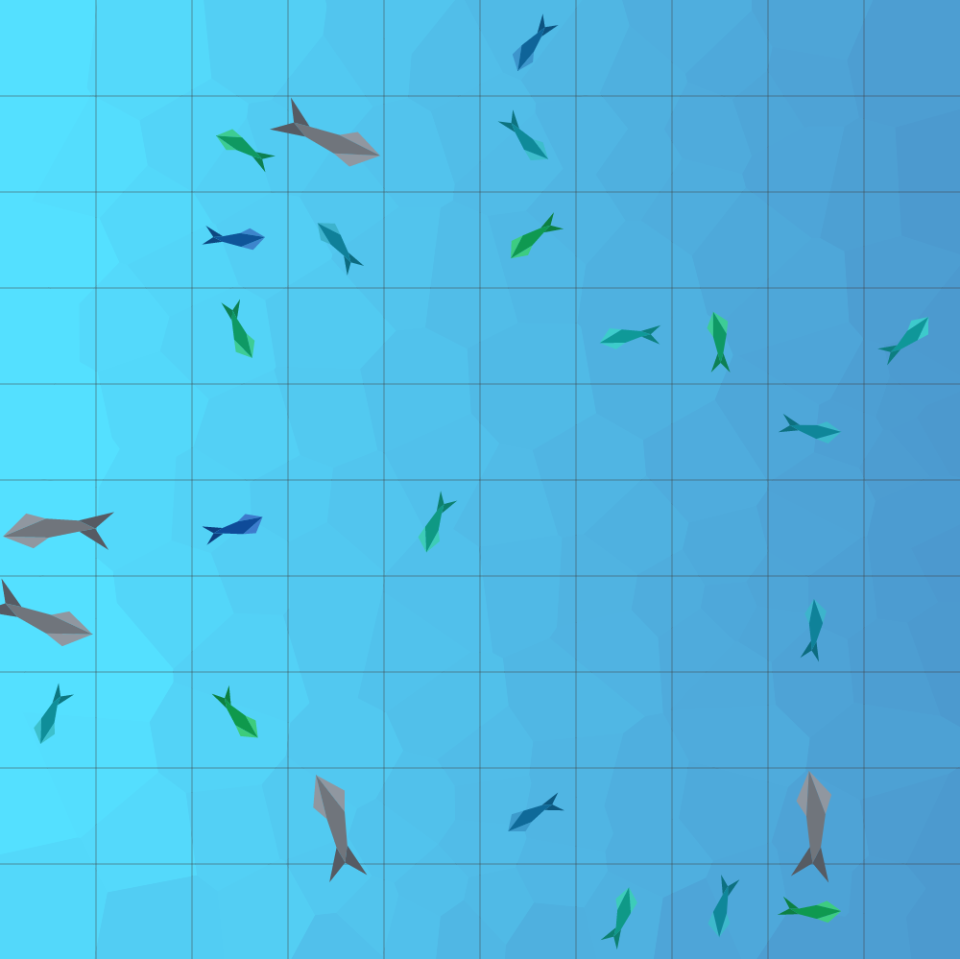
\includegraphics[width=0.6\textwidth]{pictures/classic2.png}
		\label{fig:wator}
		\caption{Ein typischer Tag auf \wator}
	\end{figure}

	\begin{figure}
		\centering
		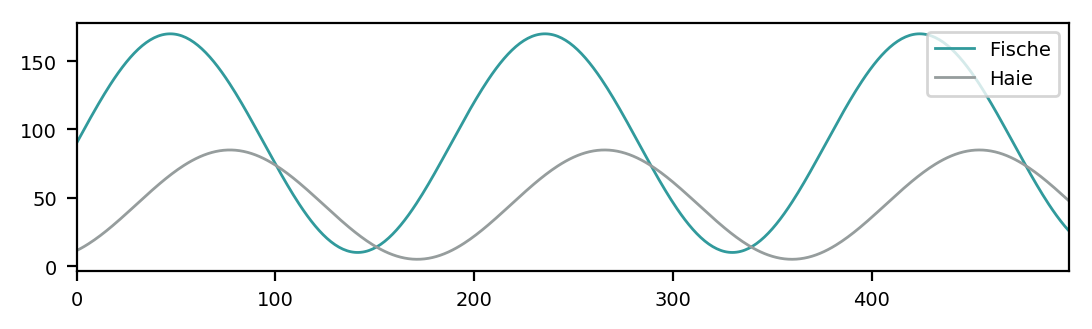
\includegraphics[width=\textwidth]{pictures/lotka_volterra.png}
		\label{fig:lotka_volterra}
		%\caption{Ein typischer Tag auf \wator}
	\end{figure}

	\begin{figure}
		\centering
		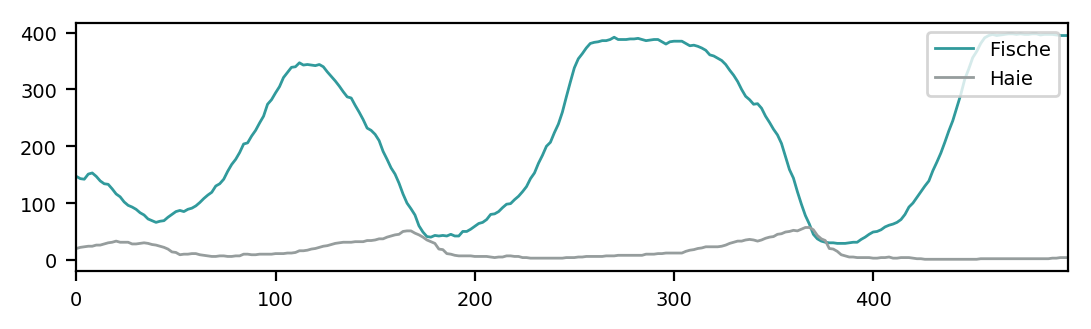
\includegraphics[width=\textwidth]{pictures/classic_default.png}
		\label{fig:classic_default}
		%\caption{Ein typischer Tag auf \wator}
	\end{figure}

	\begin{figure}
		\centering
		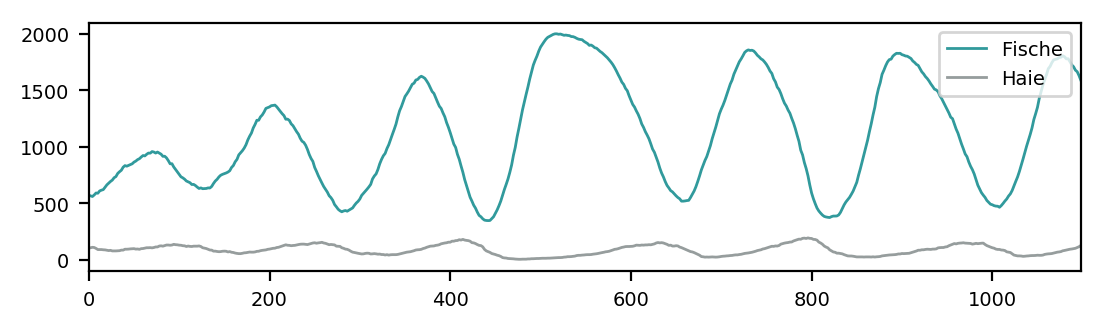
\includegraphics[width=\textwidth]{pictures/classic_big.png}
		\label{fig:classic_big}
		%\caption{Ein typischer Tag auf \wator}
	\end{figure}

	\section{Das stetige WATOR Programm}
	Im ersten Schritt ließen wir die Bewohner auf einem vordefinierten festen Gitter schwimmen. Das führt allerdings dazu, dass es eine vom Gitter induzierte natürliche Beschränkung für die Anzahl an Bewohnern gibt. Die Populationsschwankung ist somit deutlich eingeschränkt und stößt fast immer an ihre Grenzen. Ziel ist es also eine stabile Räuber-Beute-Beziehung zu modellieren, bei der im Idealfall niemand ausstirbt und die Populationsschwankung nur in Ausnahmefällen künstlich nach oben beschränkt werden muss.
	Dazu verringern wir die Gitterbreite auf ein Minimum. Somit schwimmen die Bewohner nun auf den einzelnen Pixel. Zusätzlich lassen wir zu, dass sich die Bewohner auch zur gleichen Zeit auf den selben Koordinaten befinden können.
	\begin{figure}
		\centering
		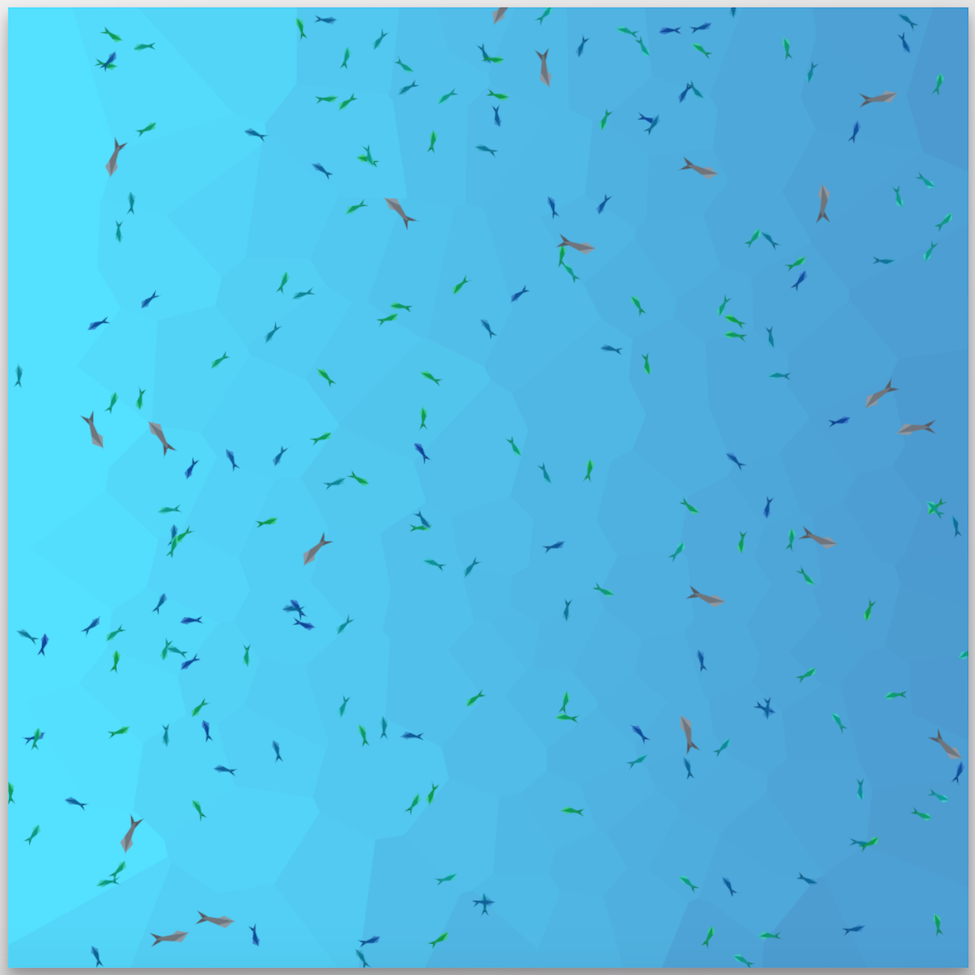
\includegraphics[width=0.7\textwidth]{pictures/continuous.png}
		\label{fig:continuous}
		\caption{Das stetige \wator}
	\end{figure}
	Diese Anpassung bringt aber einige Probleme mit sich, wie man schnell bemerkt.\newline
	
	Zunächst würden Haie nun aussterben, suchten sie nur auf den benachbarten Pixeln nach Nahrung, Sie wären also sozusagen blind und würden erst dann einen Fisch fressen, wenn er sie berührt. Deshalb definieren wir eine Suchtoleranz, sodass Haie nach Fischen suchen, die sich innerhalb dieser befinden. Findet ein Hai zum gegebenen Chrone Fische, welche sich in dieser Umgebung aufhalten, so wählt er einen dieser Fische zufällig aus und macht ihn zu seiner Nahrung.\newline
	
	Ein weiteres Problem stellen die Bewegungsabläufe dar. Zuvor ließen wir die Bewohner zufällig in eine der vier Himmelsrichtungen schwimmen. Beim stetigen \wator haben wir aber weit mehr mögliche Schwimmrichtungen. Man könnte als erstes versuchen für jedes Tier in jedem Schritt eine gleichverteilte Zufallszahl zu erzeugen, welche den Winkel der Schwimmrichtung bestimmt.
	Lässt man die Simulation nun mit diesen Änderungen laufen, so sieht das Ergebnis äußerst ernüchternd aus.
	Sowohl die Haie als auch die Fische schwimmen orientierungslos umher und bewegen sich eher wie die Nadel eines Kompasses, die von einem Magneten gestörte wird. 
	Damit diese unnatürlichen Bewegungen vermieden werden, könnte man zum Beispiel die neue Schwimmrichtung so wählen, dass sie einen zufällig gewählten aber beschränkten Winkel mit der alten Schwimmrichtung einschließt.\newline
	
	Allerdings stellen uns all diese Nachbesserungen immer noch nicht zufrieden. Die Fische schwimmen jetzt zwar natürlicher aber dennoch sehen sie recht verloren und orientierungslos aus. Wir wollen daher einen Schritt weiter gehen und die Simulation so realistisch wie möglich machen. Also implementieren wir ein Schwarmverhalten für die Fische, um sie mit ein wenig mehr Intelligenz zu versehen.
	
	\subsection{Schwarmverhalten}
	Als Modell für das Schwarmverhalten nehmen wir das verfeinerte Cucker-Smale nach ~\cite{agueh2011analysis}. 
	Die Bewegungsänderung für jedes Individuum wird dabei durch ein System von nichtlinearen Differentialgleichungen beschrieben.
	\begin{align*}
		\frac{d}{dt}x_i &= v_i\\
		\frac{d}{dt}v_i &= R^f_i + R^s_i + A_i  + B_i + (\alpha - \beta |v_i|^2)v_i,
	\end{align*}
	wobei $R^f_i$ der Abstoßungsterm für das $i$-te Individuum von den anderen Fischen, $R^s_i$ der Abstoßungsterm für das $i$-te Individuum von den Haien, $A_i$ der Anziehungsterm für das $i$-te Individuum zu den anderen Fischen, $B_i$ die Randkraft für jedes Individuum und letzter Term die Selbstantriebskraft des jeweiligen Individuums ist.\newline
	Genauer:
	\subsubsection{Selbstantrieb}	
		Der Selbstantriebsterm $(\alpha - \beta |v_i|^2)v_i$ bestimmt die Geschwindigkeit des Individuums, welche es annehmen würde, wäre kein anderes Individuum in der Nähe. Der Parameter $\alpha$ repräsentiert den Selbstantrieb des Individuums, also den Wunsch, sich
in einer gewissen Geschwindigkeit fort zu bewegen. Der Parameter $\beta$ ist hingegen ein Reibungswiderstand, der abbremsend wirkt.
		Man sieht sofort, dass
		\begin{equation}
		|v| = \sqrt{\frac{\alpha}{\beta}}
		\end{equation}
		eine stationäre Lösung von 
	\begin{equation}
		\frac{d}{dt}v_i = (\alpha - \beta |v_i|^2)v_i
		\end{equation}
		ist.
	\subsubsection{Abstoßung}
	Für das Verhalten der Fische wollen wir nicht nur, dass sie sich gegenseitig abstoßen, falls sie sich zu nahe kommen, sondern auch, dass sie in der Lage sind von Haien davon zu schwimmen, falls diese ihnen zu nahe kamen. Deswegen Verwenden wir zwei verschiedene Abstoßterme
	\begin{align*}
		R^{f,s}_i &\coloneqq \frac{\rho}{N_{f,s}}\sum^N_{j=1} S_0(|x_i-x_j|, k_{f,s}, d_{f,s})\frac{x_i-x_j}{\left(1+|x_i-x_j|^2\right)^{\gamma}},
	\end{align*}
	wobei $\rho$ und $\gamma$ die Stärke der Abstoßung bestimmen und mit einer Cutoff Funktion Abbildung \ref{fig:cutoff} für die Distanz
	\begin{align*}
		S_0(x, k, d) \coloneqq \frac{1}{2}(1-\tanh(k(x-d))),
	\end{align*}
	\begin{figure}
	\centering
	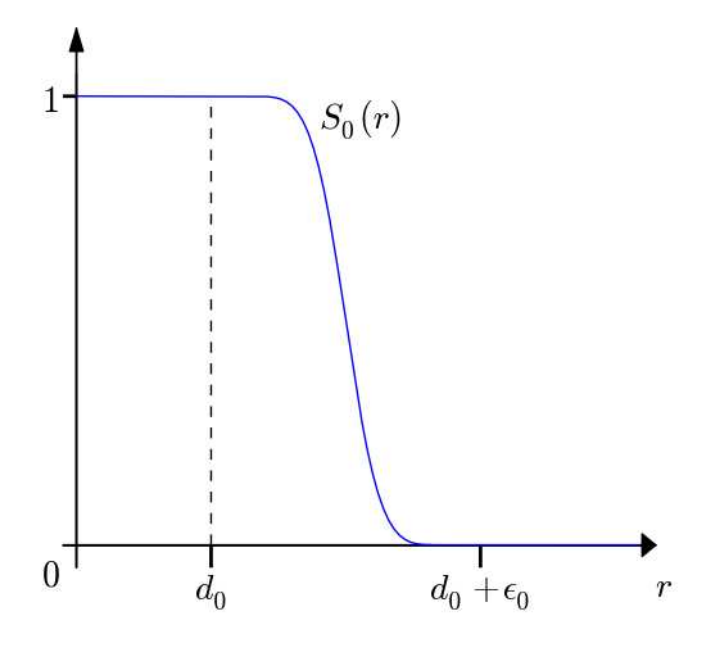
\includegraphics[width=0.4\textwidth]{pictures/cutoff.png}
		\label{fig:cutoff}
		\caption{Cutoff-Funktion \cite{agueh2011analysis}}
	\end{figure}
	wobei $d$ die Position und $k$ die Schärfe des Cutoffs bestimmt. 
Die abstoßende Kraft zwischen zwei Individuen wird dadurch abgeschnitten, wenn ihr Abstand größer als $d$ ist.

	\subsubsection{Anziehung}
	Der Term für die Anziehung ist folgendermaßen definiert:
	\begin{align*}
		A_i &\coloneqq \frac{1}{N}\sum^N_{j = 1} (1-S_0(|x_i - x_j|))w(x_i - x_j, v_i)(x_j - x_i), 
	\end{align*}
	mit Positions-Cutoff $S_0$ für die Distanz zweier Individuen und einer Funktion $w$ für den Sichtkegel
	\begin{align*}
		w(x,v) &\coloneqq \frac{\gamma}{(q+|x|^2)^{\sigma}}\left(1-(1-S_0(|v|, k_1, d_1))\cdot S_0(\frac{x\cdot v}{|x||v|}, k_2, d_2)\right),
	\end{align*}
	wobei $\gamma$ und $\sigma$ die Anziehungsstärke bestimmen und die Cutoff-Funktionen die Anziehung zum einen durch die Geschwindigkeit und zum anderen durch den Sichtkegel des Individuums abschneiden.
	Es gilt $\cos(\phi) = \frac{x\cdot v}{|x||v|}$. Ist also $\cos(\phi)$, wobei $\phi$ der Winkel zwischen Schwimmrichtung $v_i$ und dem Richtungsvektor $x_i - x_j$ zum gesehenen Individuum definiert, größer als $d_2$, der Winkel $\phi$ also klein genug, so sieht der Fisch den Anderen und der Anziehungsterm wird dazu addiert. Bei kleinen Geschwindigkeiten $|v_i| < d_1$ verschwindet die Geschwindigkeits-Cutoff-Funktion $1-S_0(|v_i|, k_1, d_1)$ und der der Sichtkegel wird ignoriert.
	
	\subsubsection{Randkräfte}
	Die Randkraft bewirkt, dass Individuen, welche sich zu weit von der Gruppe entfernt haben, ihre Richtung ändern um den Schwarm wiederzufinden.
	\begin{align*}
		B_i &\coloneqq CS_0(\rho_i, k_3, d_3)\cdot v_i^\perp, 
	\end{align*}
	mit $\rho_i = \sum^N_{j = 1} \frac{1}{1+|x_i-x_j|^2}$ und $C$ die Stärke der Randkräfte bestimmt.
	Hierbei ist $\rho_i$ ein Maß für die Einsamkeit eines Fisches. Je kleiner $\rho_i$, desto weiter befindet er sich weg vom Schwarm.
	Damit verschwindet $B_i$, falls $\rho_i > d_3$.\newline
	
	Somit wird nun in jedem Zeitschritt für jeden Fisch eine Differentialgleichung gelöst, was das ganze Unterfangen wesentlich aufwändiger macht. Wir müssen natürlich wieder eine künstliche Beschränkung für die Anzahl an Fischen definieren, da beim möglichen Aussterben der Haie und beim unendlichen Vermehren der Fische der Rechenaufwand und Speicher explodieren würde. Zusätzlich geben wir den Fischen ein Alter. Fische die ein gewisses Alter überstreichen, indem sie nicht gefressen wurden, sterben. Das macht die Differentialgleichung stabiler, da Fische hoffentlich sterben, bevor durch die Fehlerfortpflanzung Geschwindigkeiten explodieren können.\newline
	
	Im Zuge dessen müssen wir die Haie nun ebenfalls intelligenter machen, da jetzt die Chancen zufällig einen Fisch in der Nähe zu finden geringer sind. Wir lassen sie nun jagen. Zu jedem Zeitschritt sucht sich jeder Hai jeweils den zu seiner Position nächsten Fisch aus, um ihn zu jagen. In jedem Zeitschritt wird also ein neuer Fisch ausgesucht, falls der zuvor ausgewählte nicht mehr der nächste war.\newline
	
	Mit diesen Erweiterungen gelingt es tatsächlich meist stabile Populationsschwankung zu erhalten, ohne dass eine Spezies ausstirbt.
	Dabei treten Populationsverläufe (Abblindung \ref{fig:continuous_diagram}) auf, welche stark an jene der Lotka-Volterra Gleichungen erinnern.
	
	\begin{figure}
	\centering
	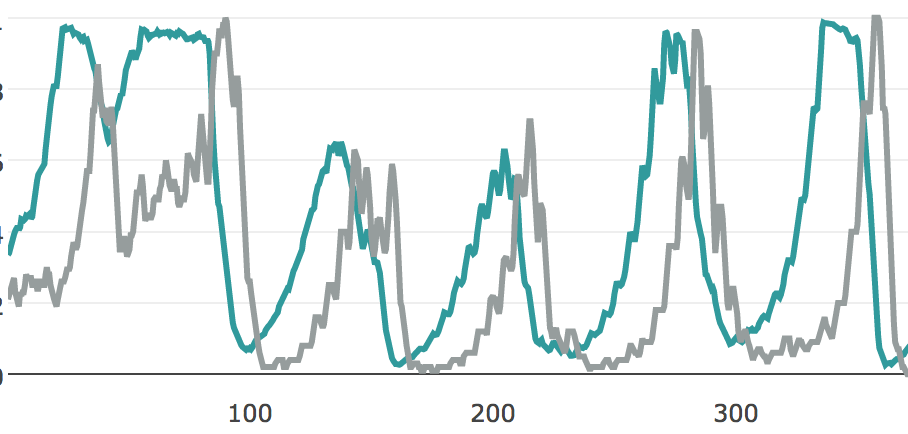
\includegraphics[width=0.7\textwidth]{pictures/continuous_diagram.png}
		\label{fig:continuous_diagram}
		\caption{Typischer Populationsverlauf beim stetigen \wator}
	\end{figure}

	\section{Animationen}
% Figures
	
	\listoffigures
	
% Literatur 


	\nocite{*}
	%\printbibliography[heading=bibintoc]% show bibliography in toc
	
\end{document}